\documentclass[a4paper,12pt, oneside]{book}

%\usepackage{fullpage}
\usepackage[italian]{babel}
\usepackage[utf8]{inputenc}
\usepackage{amssymb}
\usepackage{amsthm}
\usepackage{graphics}
\usepackage{amsfonts}
\usepackage{listings}
\usepackage{amsmath}
\usepackage{amstext}
\usepackage{engrec}
\usepackage{rotating}
\usepackage[safe,extra]{tipa}
\usepackage{showkeys}
\usepackage{multirow}
\usepackage{hyperref}
\usepackage{microtype}
\usepackage{enumerate}
\usepackage{braket}
\usepackage{marginnote}
\usepackage{pgfplots}
\usepackage{cancel}
\usepackage{polynom}
\usepackage{booktabs}
\usepackage{enumitem}
\usepackage{framed}
\usepackage{pdfpages}
\usepackage{pgfplots}
\usepackage[cache=false]{minted}
\usepackage{fancyhdr}
\pagestyle{fancy}
\fancyhead[LE,RO]{\slshape \rightmark}
\fancyhead[LO,RE]{\slshape \leftmark}
\fancyfoot[C]{\thepage}



\title{Sistemi distribuiti}
\author{UniShare\\\\Davide Cozzi\\\href{https://t.me/dlcgold}{@dlcgold}\\\\Gabriele De Rosa\\\href{https://t.me/derogab}{@derogab} \\\\Federica Di Lauro\\\href{https://t.me/f_dila}{@f\textunderscore dila}}
\date{}

\pgfplotsset{compat=1.13}
\begin{document}
\maketitle

\definecolor{shadecolor}{gray}{0.80}

\newtheorem{teorema}{Teorema}
\newtheorem{definizione}{Definizione}
\newtheorem{esempio}{Esempio}
\newtheorem{corollario}{Corollario}
\newtheorem{lemma}{Lemma}
\newtheorem{osservazione}{Osservazione}
\newtheorem{nota}{Nota}
\newtheorem{esercizio}{Esercizio}
\tableofcontents
\renewcommand{\chaptermark}[1]{%
	\markboth{\chaptername
		\ \thechapter.\ #1}{}}
\renewcommand{\sectionmark}[1]{\markright{\thesection.\ #1}}
\chapter{Introduzione}
\textbf{Questi appunti sono presi a le lezioni. Per quanto sia stata fatta una revisione è altamente probabile (praticamente certo) che possano contenere errori, sia di stampa che di vero e proprio contenuto. Per eventuali proposte di correzione effettuare una pull request. Link: } \url{https://github.com/dlcgold/Appunti}.\\
\textbf{Grazie mille e buono studio!}
\chapter{Introduzione ai Sistemi Distribuiti}
In questo corso analizziamo i sistemi distribuiti, alla base di tutte le applicazioni software 
client/server, in cui è presente una comunicazione tra diversi host.

\begin{definizione}
Un sistema distribuito è un sistema nel quale componenti hardware e software, collocati in computer
connessi alla rete, in cui comunicano e coordinano le loro azione  col passaggio di messaggi.\\
Ogni processo ha quindi una parte di logica applicativa e una parte di coordinamento. 
\end{definizione}

\begin{definizione}
un sistema distribuito è un insieme di elementi autonomi di computazione che si 
interfacciano agli utenti come un singolo sistema "coerente".
\end{definizione}

\begin{center}
	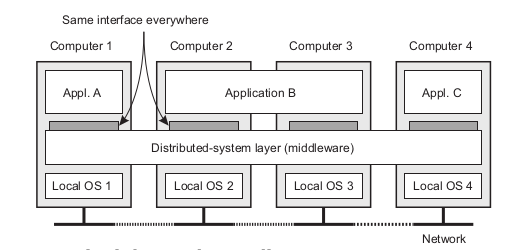
\includegraphics[scale=2.5]{img/cli.png}
\end{center}
Le unità di computazioni sono dei nodi, i quali possono essere device hardware e/o singoli processi software, autonomi che devono essere sincronizzati e coordinati(programmazione concorrente).\\ Gli utenti e le applicazioni vedono un singolo sistema, senza conoscere le varie segmentazioni e i nodi presenti, e questo permette di effettuare la \textbf{trasparenza di distribuzione}, ossia si nascondono i dettegli agli utenti che possono ignorare e non possono modificare il servizio.\newline Con la trasparenza in teoria si dovrebbe evitano la generazione degli errori, in quanto i nodi sono
indipendenti, ma in pratica tutto ciò è difficile da fare, quindi i nodi sono completamente indipendenti.

In un sistema distribuito, in quanto la comunicazione avviene tramite messaggi, non è presente la memoria
condivisa e non si ha un clock globale del sistema, ma ogni nodo si gestisce attraverso un clock interno.

\begin{center}
	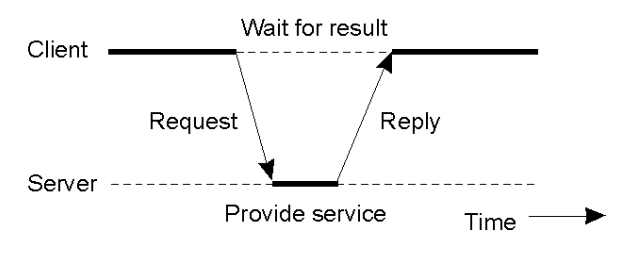
\includegraphics[scale=0.6]{img/cli2.png}
\end{center}
Si ha che un client fa una richiesta e il server risponde con un certo risultato (con il conseguente ritardo, a differenza del modello a chiamata di procedura).
\begin{center}
	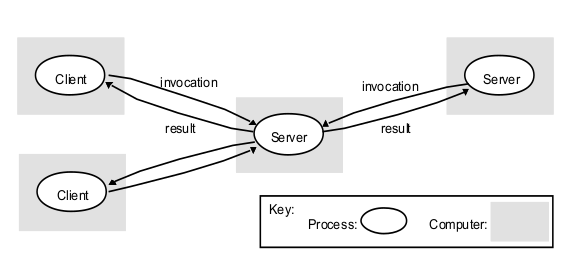
\includegraphics[scale=2.6]{img/cli3.png}
\end{center}
Si può accedere a server multipli (cluster con anche bilanciamento del carico) e si può accedere via proxy (dei server "finti" che fungono da concentratori).\\
Un sistema distribuito per comunicare effettua le seguenti operazioni:
\begin{enumerate}
    \item \textbf{identifica la controparte}, attraverso l'assegnazione di un nome(\emph{naming})
    \item \textbf{si accede alla controparte}, attraverso un punto di accesso
    \item \textbf{si definisce il protocollo}, al fine di stabilire le regole e le procedure per 
        essere in grado di comunicare, senza alcun problema.
    \item \textbf{si definisce}, che si risolve concordando \textit{sintassi e semantica} per l'informazione da condividere \textbf{(quest'ultimo è però ancora un problema aperto)}
\end{enumerate}

Si hanno le seguenti definizioni per quanto riguarda la trasparenza:
\begin{itemize}
    \item \textbf{naming}, si usano nomi simbolici per identificare le risorse,
            facenti parte del sistema distribuito.
    \item \textbf{access trasparency}, nascondere le differenze nella rappresentazione 
        delle informazioni e nell'accesso ad un'informazione locale o remota 
    \item \textbf{location trasparency}, in cui si nasconde dove è collocata una risorsa sulla rete
    \item  \textbf{relocation(mobility) transparency}, in cui si nasconde se la risorsa è stata
        trasferita ad un'altra locazione, mentre è in uso.
    \item \textbf{migration trasparency}, in cui si nasconde che una risorsa può essere trasferita
    \item \textbf{replication transparency}, in cui si nasconde che una risorsa può essere replicata
    \item \textbf{concurrency transparency}, in cui si nasconde che una risorsa può essere condivisa
        da molti utenti indipendenti
    \item \textbf{failure trasparency}, in cui si nascondono fallimenti e recovery di una risorsa
    \item \textbf{persistence trasparency}, in cui si nasconde se una risorsa
                  è volatile o memorizzata permanentemente
\end{itemize}
Da questa trasparenze non si è in grado di nascondere i ritardi e le latenze di comunicazione, ma
soprattutto non si è in grado di effettuare una trasparenza completa, per motivi di performance
e di latenza dell'operazioni su un sistema distribuito.

Questa volonta di astrarre le informazioni è alla base dell'ingegneria del software, in cui si separa
il \textit{cosa} dal \textit{come}: il cosa si effettua tramite la definizione dell'interfaccia, complete
ed indipendenti dalle diverse implementazioni, mentre il come avviene con l'effettiva implementazione
delle classi e dei metodi.\newline
Come si vede nella figura \href{figura:interfaccia}, l'interfaccia è unica mentre l'implementazione
varia in ogni host locale del sistema distribuito e ciò può essere anche visto come la separazione
tra un meccanismo e una politica, ossia come si implementa effettivamente una funzionalità del sistema.

\begin{figure}
\centering
\label{figura:interfaccia}
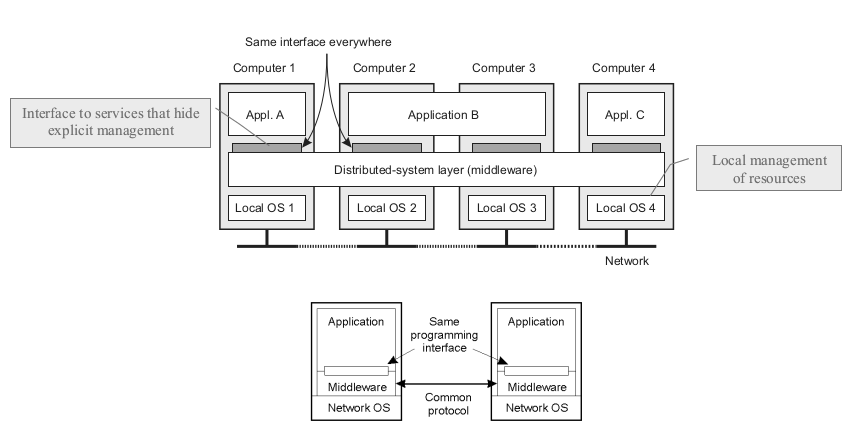
\includegraphics[scale=2]{img/cli4.png}
\end{figure}
\begin{center}
	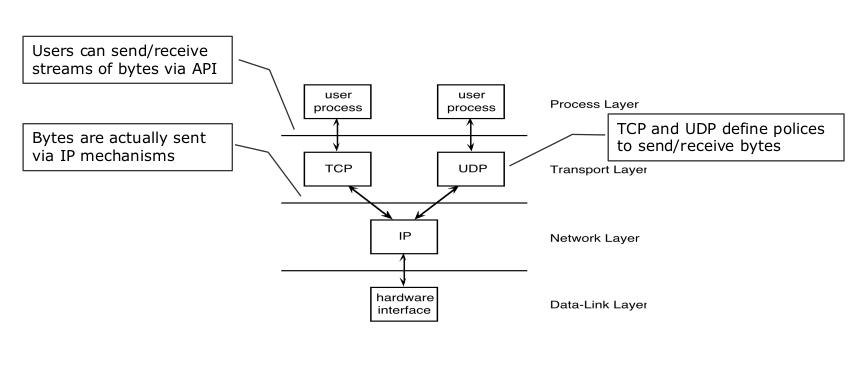
\includegraphics[scale=2]{img/cli5.png}
\end{center}
Per poter capire le richieste ed eseguire i processi di comunicazione i due processi devono concordare 
un protocollo, in cui viene definito il formato, l'ordine di invio e di ricezione dei messaggi tra 
i diversi disposizioni, e per vedere un esempio di una comunicazione tra i diversi processi si guardi
il listato di codice \href{listato:fileServer}, in cui si implementano sia l'header che l'implementazione
del server mentre nel listato di codice \href{listato:fileClient} si vede l'implementazione del client.

Non forniamo una spiegazione del codice dato che nel corso del corso impareremo come sviluppare ed
implementare applicazioni client-server.

\begin{figure}
    \label{listato:fileServer}
    \inputminted{c}{code/header.h}
    \inputminted{c}{code/fileServer.c}
\end{figure}

\begin{figure}
    \label{listato:fileClient}
    \inputminted{c}{code/fileClient.c}
\end{figure}

\subsection{Stream Communication}
\begin{figure}
    \label{figure:livelliRete}
    \centering
    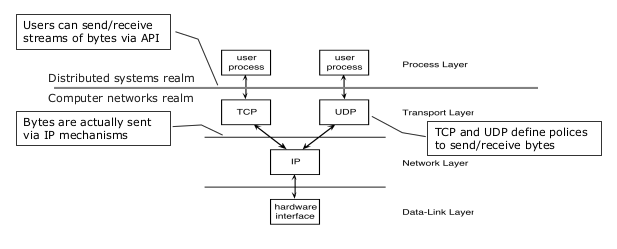
\includegraphics[scale=2.5]{img/sc.png}
\end{figure}
Per la comunicazione tra due host si utilizza il modello ISO/OSI, basato sull'astrazione di cui tutti gli
informatici ne dovrebbero conoscere in dettaglio tutti i vari livelli, in cui per mandare dei dati da un host
ad un host si parte dal livello di applicazione, su cui si sviluppano ed operano i sistemi distribuiti,
per poi andare ai livello di trasporto, di rete e fisico, necessari per il trasferimento sulla rete 
delle informazioni, come si nota nella figura \href{figure:livelliRete}.

Ogni processo comunica attraverso canali, in cui vengono gestiti i flussi di dati in ingresso ed uscita,
individuabili tramite un intero detto \textbf{porta} e noi studiamo le \textbf{socket}, particolare canale
per la comunicazione in cui non vi è una condivisione della memoria e per potersi connettere da un processo A,
il processo B deve conoscere l'host che esegue A e la porta in cui A è connesso.

Le socket possono essere principalmente di due tipi, come i principali protocolli di trasporti:
\begin{itemize}
    \item \textbf{tcp socket}: utilizzano il protocollo TCP, orientato alla connessione,
        per la comunicazione tra i due processi, prevede un controllo di affidabilità dei messaggi,
        ossia viene assicurato che i messaggi arrivano nell'ordine previsto all'altro processo
        ed infine vi è un controllo di flusso e di congestione ma non si hanno garanzie di banda e dei ritardi.

        Si utilizzano nelle applicazioni, in cui si deve avere la sicurezza dell'arrivo dei dati come ad
        esempio nel protocollo HTTP, per la comunicazione web, e nelle chat app come Telegram e Whatsapp.

    \item \textbf{udp socket}: utilizza il protocollo UDP, non affidabile e non orientato alla connessione,
        in cui viene solo garantito il trasferimento dei dati dalla rete all'applicazione e un controllo 
        minimale degli errori, cosa che lo definisce come un sottoinsieme proprio del protocollo TCP.\newline
        Viene utilizzato quando si deve avere un ritardo di trasmissione limitato ed una perdità minimale
        può non essere un problema, come ad esempio nei file multimediali e/o chiamate via voip.
\end{itemize}
Nei sistemi distribuiti non è necessario conoscere il funzionamento dei protocolli di trasporto ma basta
considerare i servizi offerti e il fatto che si trasferiscono stream di byte, infatti
le socket sono delle API(Application Programming Interface) per accedere a TCP o UDP, in quanto due processi
nel modello client-server comunicano mediante esso.

Si hanno delle criticità riguardanti alle socket e al modello client-server:
\begin{itemize}
    \item gestione del ciclo di vita di cliente e server, attivazione/terminazione del cliente e del server
    \item identificazione e accesso al server
    \item comunicazione tra client e server
    \item ripartizione dei compiti tra client e server, che dipende dal tipo di applicazioni 
          e la scelta influenza le prestazioni in relazione al carico
\end{itemize}
Quando viene definito l'indirizzo del server, esso può essere una costante, inserito dall'utente oppure
inserendo un nameserver su cui si ricava l'indirizzo tramite il DNS(Domain Name Service) e questo comporta 
un basso livello di trasparenza dato che gli utenti devono conoscre l'indirizzo della rete e soprattutto 
parsare lo stream di byte nel message voluto.

La comunicazione TCP/IP avviene attraverso flussi di byte, dopo una connessione esplicita, attraverso
normali system call read/write:queste due syscall sono sospensive, ossia mettono il sistema in attesa,
e utilizzano un buffer per garantire la massima flessibilità, ad esempio la read definisce un buffer
per leggere N caratteri ma potrebbe ritornare dopo aver letto solo $k < n$ caratteri.

\begin{figure}
\centering
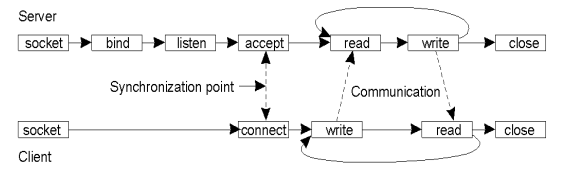
\includegraphics[scale=0.7]{img/sc2.png}
\end{figure}
\newpage
Ci sono molte chiamate diverse per accedere i servizi TCP e UDP:
\begin{center}
	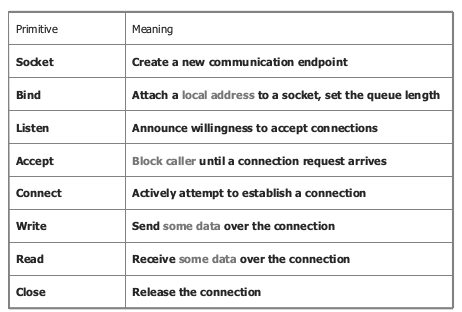
\includegraphics[scale=3]{img/sc3.png}
\end{center}
Per capire le operazioni e le procedure usate per permettere la comunicazione tra client e server,
mostriamo l'implementazione client-server con udp, nel listato \ref{udpSocket}, e quella
client-server tramite tcp, nel listato \ref{tcpSocket}.

\begin{figure}
    \caption{Implementazione socket con protocollo udp}\label{udpSocket}
    \inputminted{python}{code/udpClient.py}
    \inputminted{python}{code/udpServer.py}
\end{figure}

\begin{figure}
    \caption{Implementazione socket con protocollo tcp}\label{tcpSocket}
    \inputminted{python}{code/tcpClient.py}
    \inputminted{python}{code/tcpServer.py}
\end{figure}
Nelle socket udp, protocollo in cui si implementa un sottoinsieme delle funzionalità delle tcp, 
si effettua la creazione della socket, sia nel client che nel server, e poi subito incomincia la 
comunicazione mentre nelle socket tcp si effettua prima un handshake a tre vie per settare la connessione
tra client e server e poi incomincia la comunicazione.

Il server crea una nuova socket collegata (binded) a una nuova porta per comunicare con il client,
in questo modo la well-known port resta dedicata a ricevere richieste di connessione:
\begin{center}
	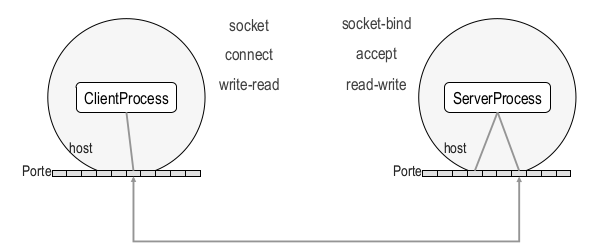
\includegraphics[scale=3]{img/sc4.png}
\end{center}
\begin{minted}{c}
byteLetti read(socket, buffer, dimBuffer);
\end{minted}
con:
\begin{itemize}
	\item byteLetti = byte effettivamente letti
	\item socket = canale da cui leggere
	\item buffer = sapzio di memoria dove trasferire i byte letti
	\item dimBuffer = dimensione del buffer = numero max di caratteri che si possono leggere
\end{itemize}

Dopo aver mostrato come si implementano le socket in Python, per rendere semplice e facilmente comprensibile
quali sono le funzionalità e come si definiscono le socket, analizziamo come vengono fatte con il linguaggio
Java, usato nel corso, utilizzandoalcune classi che costituiscono un'interfaccia ad oggetti 
delle system call, su cui sono definite tutte le operazioni delle socket:
\begin{minted}{java}
    java.net.Socket
    java.net.ServerSocket
\end{minted}
Queste classi accorpano funzionalità e mascherano alcuni dettagli con il vantaggio di semplificarne l'uso
e come ogni framework è necessario conoscerne il modello e il funzionamento per poterlo usare efficacemente. 

I costrutti principali di queste due classi si possono trovare facilmente nella documentazione Java 
e negli esempi fatti a lezione, trovabili facilmente sul corso elearning.

Vediamo ora un esempio di un server \ref{java:tcpServer}, scritto in Java che accetta una connessione da un client 
e manda uno stream di dati, e di un client \ref{java:tcpClient}che legge lo stream di bytes, 
con un esempio similare a quello fatto in python per spiegare le fasi del TCP socket.

\begin{figure}
    \caption{Semplice implementazione TCP server in Java}
    \label{java:tcpServer}
    \inputminted{java}{code/javaSocket/ServerWriter/SenderServerSocket.java}
\end{figure}

\begin{figure}
    \caption{Semplice implementazione TCP client in Java}
    \label{java:tcpClient}
    \inputminted{java}{code/javaSocket/ServerWriter/ReceiverClientSocket.java}
\end{figure}

Quindi per il server si avrà la situazione \ref{img:javaServer} mentre nel client 
si verifica \ref{img:javaClient}.

Si nota facilmente che il seguente modello di client non funziona nella maniera corretta, per cui
si introducono i \textbf{lazy server} che mandano pochi byte per volta con un piccolo ritardo,
come si nota nel listato \ref{java:lazyServer}

\begin{center}
	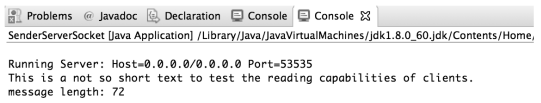
\includegraphics[scale=2.5]{img/sc5.png}
\end{center}
e per il client:
\begin{center}
	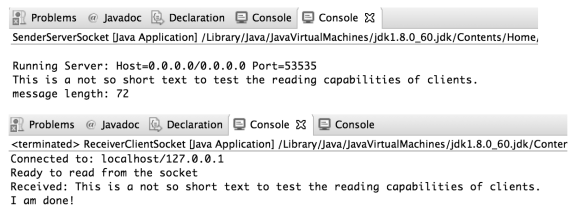
\includegraphics[scale=2.5]{img/sc6.png}
\end{center}

\begin{figure}
    \caption{Implementazione server Lazy}
    \label{java:lazyServer}
    \inputminted{java}{code/JavaSocket/ServerWriter/LazySenderServerSocket.java}
\end{figure}

\begin{center}
	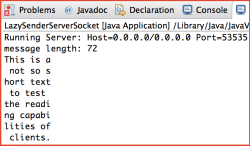
\includegraphics[scale=0.7]{img/lazy.png}
\end{center}
Per un'applicazione socket si ha le seguenti componenti:
\begin{enumerate}
	\item \textbf{client} con l'architettura che è concettualmente più semplice di quella di un server,
        spesso è un'applicazione convenzionale in cui si hanno solo effetti sull'utente client 
        e non comporta problemi di sicurezza.
	\item \textbf{server}: crea una socket, gli assegna una porta nota ed entra in ciclo infinito 
        in cui alternare: attesa di una richiesta, soddisfo la richiesta ed invio la risposta.\newline
	    L'affidabilità di un server è strettamente dipendente dall'affidabilità della comunicazione 
        tra lui e i suoi client, del resto però la modalità \textit{connection-oriented} determina 
        l'impossibilità di rilevare interruzioni sulle connessioni e la necessità di prevedere 
        una connessione (una socket) per ogni comunicazione.
\end{enumerate}
Ci sono diverse tipologie di server implementabili in un modello client-server:
\begin{itemize}
	\item \textbf{iterativi}, in cui viene soddisfatta una richiesta alla volta
	\item \textbf{concorrenti processo singolo}, in cui viene simulata la presenza di un server dedicato
	\item \textbf{concorrenti multi-processo}, in cui vengono creati server dedicati ad ogni client.
	\item \textbf{concorrenti multi-thread}, in cui vengono creati dei threat specifici per ogni client.
\end{itemize}
Vediamo come progettare un server iterativo. Al momento di una richiesta di connessione il server crea una
socket temporanea per stabilire una connessione diretta con il client Le eventuali ulteriori richieste per il server verranno accodate alla porta nota per essere successivamente soddisfatte. Si hanno degli svantaggi:
\begin{itemize}
	\item viene servito un cliente alla volta, gli altri devono attendere
	\item un server impedisce l'evoluzione di molti client
	\item non scala
\end{itemize}
La soluzione sono i \textit{server concorrenti}.\\
Vediamo un esempio di un server che semplicemente legge da una socker e scrive sulla console:
\begin{minted}{java}
package SelectorExample;

import java.io.DataInputStream;
import java.net.ServerSocket;
import java.net.Socket;

public class IterativeServer {

  public static void main(String[] args) {
    ServerSocket listenSocket;
    Socket clientSocket;
    byte[] byteReceived = new byte[1000];
    String messageString = "";

    try {
      listenSocket = new ServerSocket(53535);
      System.out.println("*** Running Server: " + "Host=" + listenSocket.getInetAddress() + " Port="
          + listenSocket.getLocalPort());

      while (true) {
        clientSocket = listenSocket.accept();

        DataInputStream in = new DataInputStream(clientSocket.getInputStream());
        int bytesRead = 0;

        while (true) {
          bytesRead = in.read(byteReceived);
          if (bytesRead == -1)
            break; // no more bytes
          messageString += new String(byteReceived, 0, bytesRead);
          System.out.println("Received: " + messageString);
        }

        clientSocket.close();
        messageString = ""; // clear the string for the next client
        System.out.println("*** Avaialble to the next client.");
      }
    } catch (Exception e) {
      e.printStackTrace();
    }
  }
}

\end{minted}
\newpage

Un server concorrente può gestire più connessioni client.
\begin{center}
	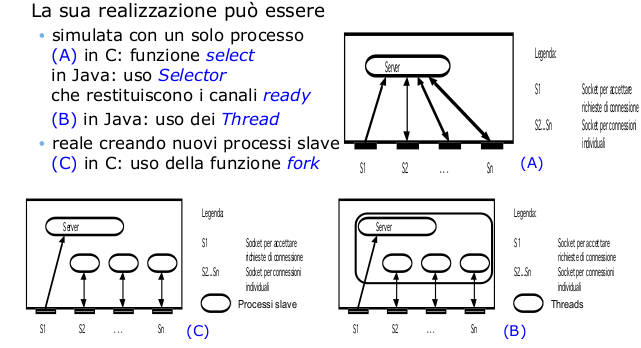
\includegraphics[scale=2.7]{img/conc.png}
\end{center}
In java si ha anche il \textbf{multiplexing} dove:
\begin{itemize}
	\item i \textbf{channel} possono operare sia in modalità bloccante che non bloccante. In modalità non bloccante (dove solo canali stream-oriented, come socket e pipe, possono essere usati) il channel non mette mai il thread invocato in sleep. L'operazione richiesta o viene completata completamente o ritorna che nulla è stato fatto
	\item si hanno classi speciali per java, come \textit{ServerSocketChannel, SocketChannel e
		      DatagramChannel} e si usano i selector, permettendo un controllo più fine dei socket channels.
\end{itemize}
Un Selector è un multiplexort di oggetti \textit{SelectableChannel} e viene creato con:
\begin{minted}{java}
Selector selector = Selector.open();
\end{minted}
I selector vengono poi registrati col metodo \textit{register}:
\begin{minted}{java}
channel.configureBlocking(false);
SelectionKey key = channel.register(selector, SelectionKey.OP_READ);
\end{minted}
Con le seguenti \textit{SelectionKey}:
\begin{minted}{java}
SelectionKey.OP_CONNECT // quando un client tenta di connettersi al server
SelectionKey.OP_ACCEPT // quando il server accetta la connessione del client
SelectionKey.OP_READ // quando il server è pronto a leggere dal canale
SelectionKey.OP_WRITE // quando il server è pronto a scrivere sul canale
\end{minted}
In generale ecco lo pseudo-codice per un server non bloccante:
\begin{verbatim}
create SocketChannel;
create Selector;
associate the SocketChannel with the Selector;
while(true) {
  waiting events from the Selector;
  event arrived;
  create keys;
  for each key created by Selector {
    check the type of request;
    isAcceptable:
      get the client SocketChannel;
      associate that SocketChannel with the Selector;
      record it for read/write operations
      continue;
    isReadable:
      get the client SocketChannel;
      read from the socket;
      continue;
    isWriteable:
      get the client SocketChannel;
      write on the socket;
      continue;
  }
}
\end{verbatim}
\newpage
ovvero:
\begin{center}
	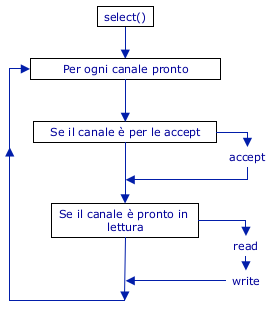
\includegraphics[scale=2.7]{img/conc2.png}
\end{center}
In java:
\begin{minted}{java}
import java.io.IOException;
import java.io.PrintWriter;
import java.net.InetAddress;
import java.net.Socket;
import java.util.Scanner;

public class SenderClient {
  private Socket socket;
  private Scanner scanner;

  private SenderClient(InetAddress serverAddress, 
    int serverPort) throws Exception {
    this.socket = new Socket(serverAddress, serverPort);
    this.scanner = new Scanner(System.in);
  }

  private void start() throws IOException, InterruptedException {
    String input;
    PrintWriter out = new PrintWriter(this.socket.getOutputStream(), true);
    while (true) {
      input = scanner.nextLine();
      if (input.contentEquals("exit"))
          break;
      out.print(input);
      out.flush();
    }
    System.out.println("Client terminate.");
    socket.close();
  }

  public static void main(String[] args) throws Exception {
    SenderClient client = new SenderClient(InetAddress.getByName(args[0]),
        Integer.parseInt(args[1]));

    System.out.println("Connected to: " + client.socket.getInetAddress());
    client.start();

  }

}

\end{minted}
\begin{center}
	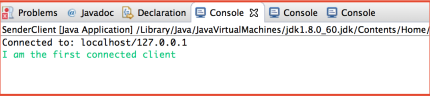
\includegraphics[scale=0.7]{img/conc4.png}
\end{center}
Vediamo come farlo in modo concorrente:
\begin{minted}{java}
package SelectorExample;

import java.io.IOException;
import java.net.InetSocketAddress;
import java.nio.ByteBuffer;
import java.nio.CharBuffer;
import java.nio.channels.SelectionKey;
import java.nio.channels.Selector;
import java.nio.channels.ServerSocketChannel;
import java.nio.channels.SocketChannel;
import java.nio.charset.Charset;
import java.nio.charset.CharsetDecoder;
import java.util.Iterator;
import java.util.Set;

public class ConcurrentServer {

  public static void main(String[] args) throws IOException {
    Selector selector = Selector.open();
    ServerSocketChannel server = ServerSocketChannel.open();
    server.bind(new InetSocketAddress("localhost", 53535));
    // set the channel in non blocking mode
    server.configureBlocking(false);
    // register the channel with the selector or the accept operation
    server.register(selector, SelectionKey.OP_ACCEPT);

    // Infinite server loop
    while (true) {
      // Waiting for events
      selector.select();
      // Get keys
      Set<SelectionKey> keys = selector.selectedKeys();
      Iterator<SelectionKey> i = keys.iterator();

      // For each keys...
      while (i.hasNext()) {
        SelectionKey key = (SelectionKey) i.next();

        // Remove the current key
        i.remove();

        if (key.isAcceptable()) // a client required a connection
          acceptClientRequest(selector, server);

        if (key.isReadable()) // ready to read
          readClientBytes(key);
      }
    }
  }

  private static void acceptClientRequest(Selector selector,
     ServerSocketChannel server) throws IOException {
    // get client socket channel
    SocketChannel client = server.accept();
    // Non Blocking I/O
    client.configureBlocking(false);
    // recording to the selector (reading)
    client.register(selector, SelectionKey.OP_READ);
    return;
  }

  private static void readClientBytes(SelectionKey key) throws IOException {
    SocketChannel client = (SocketChannel) key.channel();

    // Read byte coming from the client
    int BUFFER_SIZE = 256;
    ByteBuffer buffer = ByteBuffer.allocate(BUFFER_SIZE);
    try {
      if (client.read(buffer) == -1) {
        client.close();
        return;
      }
    } catch (Exception e) {
      // client is no longer active
      e.printStackTrace();
      client.close();
      return;
    }

    // Show bytes on the console
    buffer.flip(); // set the limit to the current position and then set 
      the position to zero 
    Charset charset = Charset.forName("UTF-8");
    CharsetDecoder decoder = charset.newDecoder();
    CharBuffer charBuffer = decoder.decode(buffer);
    int port = client.socket().getPort();
    System.out.println(port + ": " + charBuffer.toString());
    return;
  }
}

\end{minted}
\begin{center}
	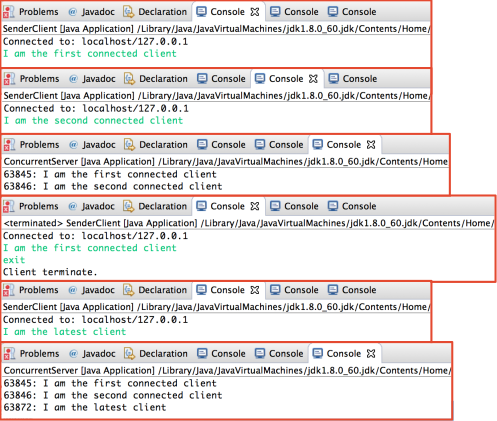
\includegraphics[scale=3]{img/conc5.png}
\end{center}
Vediamo anche una rappresentazione della chiamata di sistema fork:
\begin{center}
	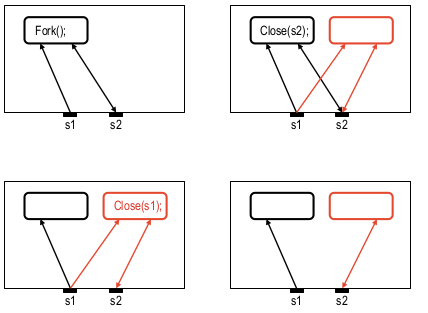
\includegraphics[scale=0.7]{img/fork.png}
\end{center}
La lettura/scrittura su una socket da parte di più processi
determina un problema di concorrenza: accesso ad una
risorsa condivisa (mutua esclusione). Si ha quindi;
\begin{center}
	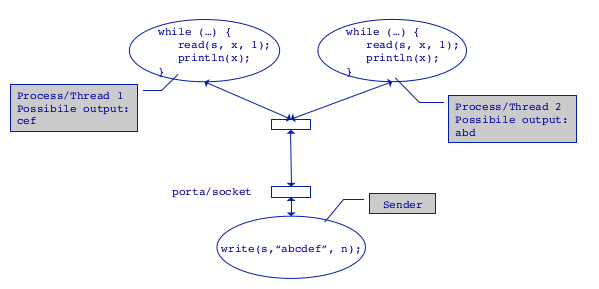
\includegraphics[scale=0.7]{img/ex.png}
\end{center}
Si hanno quindi 2 modelli:
\begin{enumerate}
	\item \textbf{mono processo (iterativo e concorrente)}, dove gli utenti condividono lo stesso spazio di lavoro. È adatto ad applicazioni cooperative che prevedono la modifica
	      dello stato (lettura e scrittura)
	\item \textbf{multi processo}, dove ogni utente ha uno spazio di lavoro autonomo. È adatto ad applicazioni autonome o che non modificano lo stato del server (sola lettura)
\end{enumerate}




















\subsection{Architettura dei server}
Per la gestione dei thread (che in java sono classi) esistono diversi \textbf{design pattern}:
\begin{itemize}
	\item \textbf{un thread per pattern}, dove il \textit{thread coordinatore} rileva la presenza di un nuovo client, lo connette ad un nuovo thread il quale:
	      \begin{itemize}
		      \item decodifica la richiesta
		      \item chiama la funzione servente che la soddisfa
		      \item torna in ciclo per leggere una nuova richiesta
	      \end{itemize}
	      \textbf{un thread per richiesta}, dove un \textit{thread coordinatore} riceve una richiesta e genera un thread per processarla. Questo nuovo thread:
	      \begin{itemize}
		      \item decodifica la richiesta
		      \item chiama la funzione servente che la soddisfa
		      \item termina
	      \end{itemize}
	\item \textbf{un thread per servente}, dove ogni servente ha un proprio thread e una coda. Il coordinatore riceve una richiesta e lo inserisce nella coda del servente giusto. Ogni thread servente legge ciclicamente una richiesta dalla
	      propria coda e la esegue
	\item \textbf{una pool di thread}, dove, dato che la creazione di un thread è costosa, il costo viene ammortizzato facendo gestire ad ogni thread molte richieste. Questo \textit{pool di thread} viene creato all'avvio del sistema e le richieste gli vengono assegnate man mano.
\end{itemize}
\subsection{Un esempio}
Vediamo un esempio client/server con socket TCP/IP in Java.\\
\textit{Vogliamo realizzare un semplice programma per giocare a “knock knock”, il popolare gioco di parole inglese che si basa su domande e risposte con parole ed espressioni omofone di significato differente:}\\
\textit{Server: "Knock knock!"\\
	Client: "Who's there?"\\
	Server: "Atch."\\
	Client: "Atch who?"\\
	Server: "Bless you!"}
\\
Facciamo quindi tre classi (\textit{qui il ruolo attivo viene assunto dal server che inizia la
	conversazione (in pratica un'inversione dei ruoli)}):
\begin{enumerate}
	\item una \textbf{classe \textit{KnockKnockProtocol}} che fornisce il protocollo, stabilendo domande e risposte e funzione la soluzione per formulare le risposte
	\item una \textbf{classe \textit{KnockKnockClient}} che stabilisce la connessione e invia i messaggi al server
	\item una \textbf{classe \textit{KnockKnockServer}} che accetta la connessione e interroga il client secondo il protocollo della prima classe
\end{enumerate}
\newpage
Vediamo la \textbf{\textit{KnockKnockServer}}:
\begin{minted}{java}
package KnockKnock;
import java.io.BufferedReader;
import java.io.IOException;
import java.io.InputStreamReader;
import java.io.PrintWriter;
import java.net.ServerSocket;
import java.net.Socket;

public class KnockKnockServer {
  public static void main(String[] args) throws IOException {
        ServerSocket serverSocket = null;
        try {
            serverSocket = new ServerSocket(4444);
        } catch (IOException e) {
            e.printStackTrace();
            System.err.println("Could not listen on port: 4444.");
            System.exit(1);
        }
        Socket clientSocket = null;
        try {
            clientSocket = serverSocket.accept();
        } catch (IOException e) {
            System.err.println("Accept failed.");
            System.exit(1);
        }
        PrintWriter out = 
          new PrintWriter(clientSocket.getOutputStream(), true);
        BufferedReader in = new BufferedReader(
        new InputStreamReader(
        clientSocket.getInputStream()));
        String inputLine, outputLine;
        KnockKnockProtocol kkp = new KnockKnockProtocol();

        outputLine = kkp.processInput(null);
        out.println(outputLine);

        while ((inputLine = in.readLine()) != null) {
             outputLine = kkp.processInput(inputLine);
             out.println(outputLine);
             if (outputLine.equals("Bye."))
                break;
        }
        out.close();
        in.close();
        clientSocket.close();
        serverSocket.close();
  }
}

\end{minted}
passiamo al client:
\begin{minted}{java}
package KnockKnock;

import java.io.BufferedReader;
import java.io.IOException;
import java.io.InputStreamReader;
import java.io.PrintWriter;
import java.net.Socket;
import java.net.UnknownHostException;

public class KnockKnockClient {

  public static void main(String[] args) throws IOException {
    Socket kkSocket = null;
    PrintWriter out = null;
    BufferedReader in = null;

    try {package KnockKnock;

public class KnockKnockProtocol {
    private static final int WAITING = 0;
    private static final int SENTKNOCKKNOCK = 1;
    private static final int SENTCLUE = 2;
    private static final int ANOTHER = 3;

    private static final int NUMJOKES = 5;

    private int state = WAITING;
    private int currentJoke = 0;

    private String[] clues = { "Turnip", "Little Old Lady", "Atch", "Who", "Who" };
    private String[] answers = { "Turnip the heat, it's cold in here!",
                                 "I didn't know you could yodel!",
                                 "Bless you!",
                                 "Is there an owl in here?",
                                 "Is there an echo in here?" };

    public String processInput(String theInput) {
        String theOutput = null;

        if (state == WAITING) {
            theOutput = "Knock! Knock!";
            state = SENTKNOCKKNOCK;
        } else if (state == SENTKNOCKKNOCK) {
            if (theInput.equalsIgnoreCase("Who's there?")) {
                theOutput = clues[currentJoke];
                state = SENTCLUE;
            } else {
                theOutput = "You're supposed to say \"Who's there?\"! " +
			    "Try again. Knock! Knock!";
            }
        } else if (state == SENTCLUE) {
            if (theInput.equalsIgnoreCase(clues[currentJoke] + " who?")) {
                theOutput = answers[currentJoke] + " Want another? (y/n)";
                state = ANOTHER;
            } else {
                theOutput = "You're supposed to say \"" + 
			    clues[currentJoke] + 
			    " who?\"" + 
			    "! Try again. Knock! Knock!";
                state = SENTKNOCKKNOCK;
            }
        } else if (state == ANOTHER) {
            if (theInput.equalsIgnoreCase("y")) {
                theOutput = "Knock! Knock!";
                if (currentJoke == (NUMJOKES - 1))
                    currentJoke = 0;
                else
                    currentJoke++;
                state = SENTKNOCKKNOCK;
            } else {
                theOutput = "Bye.";
                state = WAITING;
            }
        }
        return theOutput;
    }

}

      kkSocket = new Socket("localhost", 4444);
      out = new PrintWriter(kkSocket.getOutputStream(), true);
      in = new BufferedReader(new InputStreamReader(kkSocket.getInputStream()));
    } catch (UnknownHostException e) {
      System.err.println("Don't know about host: taranis.");
      System.exit(1);
    } catch (IOException e) {
      System.err.println("Couldn't get I/O for the connection to: taranis.");
      System.exit(1);
    }

    BufferedReader stdIn = new BufferedReader(new InputStreamReader(System.in));
    String fromServer;
    String fromUser;

    while ((fromServer = in.readLine()) != null) {
      System.out.println("Server: " + fromServer);
      if (fromServer.equals("Bye."))
        break;

      fromUser = stdIn.readLine();
      if (fromUser != null) {
        System.out.println("Client: " + fromUser);
        out.println(fromUser);
      }
    }

    out.close();
    in.close();
    stdIn.close();
    kkSocket.close();
  }

}


\end{minted}
e il server:
\begin{minted}{java}
package KnockKnock;

public class KnockKnockProtocol {
    private static final int WAITING = 0;
    private static final int SENTKNOCKKNOCK = 1;
    private static final int SENTCLUE = 2;
    private static final int ANOTHER = 3;

    private static final int NUMJOKES = 5;

    private int state = WAITING;
    private int currentJoke = 0;

    private String[] clues = { "Turnip", "Little Old Lady",
       "Atch", "Who", "Who" };
    private String[] answers = { "Turnip the heat, it's cold in here!",
                                 "I didn't know you could yodel!",
                                 "Bless you!",
                                 "Is there an owl in here?",
                                 "Is there an echo in here?" };

    public String processInput(String theInput) {
        String theOutput = null;

        if (state == WAITING) {
            theOutput = "Knock! Knock!";
            state = SENTKNOCKKNOCK;
        } else if (state == SENTKNOCKKNOCK) {
            if (theInput.equalsIgnoreCase("Who's there?")) {
                theOutput = clues[currentJoke];
                state = SENTCLUE;
            } else {
                theOutput = "You're supposed to say \"Who's there?\"! " +
          "Try again. Knock! Knock!";
            }
        } else if (state == SENTCLUE) {
            if (theInput.equalsIgnoreCase(clues[currentJoke] + " who?")) {
                theOutput = answers[currentJoke] + " Want another? (y/n)";
                state = ANOTHER;
            } else {
                theOutput = "You're supposed to say \"" + 
          clues[currentJoke] + 
          " who?\"" + 
          "! Try again. Knock! Knock!";
                state = SENTKNOCKKNOCK;
            }
        } else if (state == ANOTHER) {
            if (theInput.equalsIgnoreCase("y")) {
                theOutput = "Knock! Knock!";
                if (currentJoke == (NUMJOKES - 1))
                    currentJoke = 0;
                else
                    currentJoke++;
                state = SENTKNOCKKNOCK;
            } else {
                theOutput = "Bye.";
                state = WAITING;
            }
        }
        return theOutput;
    }

}


\end{minted}
I vari client sono quindi serviti in sequenza, con i conseguenti problemi di performance. Per servire più client in modo concorrente si unsano i server multi-thread:
\begin{verbatim}
while (true) {
 accept a connection ;
 create a thread to deal with the client ;
end while
\end{verbatim}

Si hanno due classi:
\begin{enumerate}
	\item \textbf{KKMultiServer} per i server
	\item \textbf{KKMultiServerThread} che realizza un server dedicato ad un client
\end{enumerate}
\begin{minted}{java}
package KnockKnock;

import java.io.BufferedReader;
import java.io.IOException;
import java.io.InputStreamReader;
import java.io.PrintWriter;
import java.net.ServerSocket;
import java.net.Socket;

public class KKMultiServer {

  public static class KKMultiServerThread extends Thread {
    private Socket socket = null;

    public KKMultiServerThread(Socket socket) {
      super("KKMultiServerThread");
      this.socket = socket;
    }

    public void run() {
      try {
        PrintWriter out = new PrintWriter(socket.getOutputStream(), true);
        BufferedReader in = 
          new BufferedReader(new InputStreamReader(socket.getInputStream()));
        String inputLine, outputLine;
        KnockKnockProtocol kkp = new KnockKnockProtocol();
        outputLine = kkp.processInput(null);
        out.println(outputLine);
        while ((inputLine = in.readLine()) != null) {
          outputLine = kkp.processInput(inputLine);
          out.println(outputLine);
          if (outputLine.equals("Bye"))
            break;
        }
        out.close();
        in.close();
        socket.close();
      } catch (IOException e) {
        e.printStackTrace();
      }
    }
  }

  public static void main(String[] args) {
    ServerSocket serverSocket = null;
    boolean listening = true;

    try {
      serverSocket = new ServerSocket(4444);

      while (listening)
        new KKMultiServerThread(serverSocket.accept()).start();
      serverSocket.close();
    } catch (IOException e) {
      System.err.println("Could not listen on port: 4444.");
      System.exit(-1);
    }

  }

}

\end{minted}

\section{L'architettura del web}
Per comunicare attraverso internet si utilizza un modello client-server usando principalmente 
il protocollo \textbf{HTTP}, attraverso l'esecuzione delle sue operazioni \textbf{request} e \textbf{response}:
la prima indica la richiesta di un oggetto web, come ad esempio un immagine e un file html, 
da parte del client verso il server mentre la seconda è la risposta da parte del server verso il client.

Nell'architettura di Internet il client viene realizzato mediante un browser, come ad esempio firefox,
programma che fornisce la possibilità di navigare sul web, attraverso l'interpretazione del codice
con cui sono espresse le pagine web, costituita da diversi oggetti identificati da un URL, mentre
il server viene fornito da un Web Server, come ad esempio Apache.

L'URL identifica un oggetto nella rete e specifica come interpretare i dati ricevuti 
attraverso il protocollo, è formato dai seguenti elementi:
\begin{itemize}
    \item nome del protocollo 
    \item indirizzo IP dell'host
    \item porta del processo
    \item cammino/percorso dell'host
    \item identificatore della risposta
\end{itemize}
rappresentata nel seguente modo
\begin{verbatim}
    protocollo://indirizzo_IP[:porta]/cammino/risorsa
\end{verbatim}
La parte testuale dei documenti viene espressa da HTML, per contenuti ed impaginazione, da CSS per 
il rending grafico mentre attraverso XML e JSON specifichiamo i dati e la loro struttura nel documento.

Si possono avere anche dati multimediali (foto, audio, etc...) con l'encoding MIME per definirne 
il formato (plain, html per i testi, jpeg, gif per le immagini, etc..) mentre la dinamicità delle pagine web
viene data da linguaggi di programmazione come Javascript, VBScript, Java/applet \dots .

Vi sono diversi protocolli web, in cui si definiscono le regole di comunicazioni tra varie tipologie di
applicazioni, come ad esempio HTTP, FTP(File Transfer Protocol) e SMTP(Simple Mail Transfer Protocol);
questi esempi di protocolli utilizzano il protocollo di trasporto TCP ed utilizzano delle porte note:
80 per HTTP, 20 per FTP e 25 per SMTP.

Per ora si hanno due versioni del protocollo HTTP, definite in maniera standard:
\begin{enumerate}
	\item\textbf{ http1.0: RFC 1945}
	\item\textbf{ http1.1: RFC 2068}
\end{enumerate}
HTTP è \textbf{stateless} in quanto il server non mantiene informazioni sulle precedenti richieste,
per cui si devono sempre fornire le informazioni necessarie per cui i siti web per avere informazioni 
utilizzano i cookie, che analizzeremo alla fine di questo paragrafo.\newline
Si ha che le \textit{request}e \textit{response} hanno la stessa struttura, in ASCII con un 
formato testo leggibile, ad esempio:
\begin{verbatim}
GET /somedir/page.html HTTP/1.1
Host: www.someschool.edu
Connection: close
User-agent: Mozilla/4.0
Accept: text/html, image/gif, image/jpeg
Accept-language: fr
\end{verbatim}
Con la prima riga si rappresenta la request line mentre nelle altre sono rappresentati l'header con le opzioni.

Nel protocollo HTTP si hanno diverse tipologie di metodi e richieste, le principali sono le seguenti:
\begin{itemize}
	\item \textbf{GET}: metodo HTTP, in cui viene restituita una rappresentazione di una risorsa web,
        senza effetti sul server, utile per ottenere pagine html ed immagini.

    \item \textbf{POST}: metodo HTTP, in cui vengono comunicati i dati da far elaborare al server oppure
        si crea una nuova risorsa, subordinata all'URL.\newline
        Ogni richiesta POST causa degli effetti sul server, quindi non può venire gestita la richiesta da 
        una cache e l'utilizzo tipico è quello per processare delle FORM html e di modificare 
        dati presenti in un database.
    
    \item \textbf{HEAD}: viene utilizzato spesso in fase di debugging ed è similare al metodo get
        ma in questo metodo viene restituito soltanto l'head della pagina web.
\end{itemize}
Nel complesso tutte le tipologie di richieste HTTP si notano nella figura \ref{fig:httpMethod} mentre 
il formato di una richiesta http si vede nella figura \ref{fig:httpStructure}.

\begin{figure}
    \caption{Tipologie di richieste HTTP}
    \label{fig:httpMethod}
	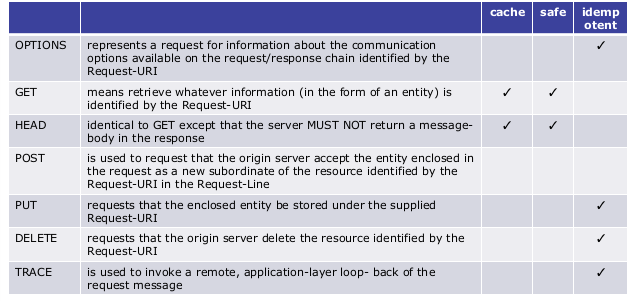
\includegraphics[scale=0.7]{img/http.png}
\end{figure}

\begin{figure}
    \caption{Formato di una richiesta HTTP}
    \label{fig:httpStructure}
	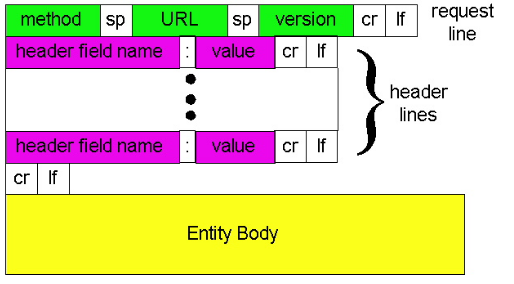
\includegraphics[scale=0.7]{img/http2.png}
\end{figure}
vediamo ora un esempio di risposta http:
\begin{verbatim}
HTTP/1.1 200 OK
Connection: close
Date: Thu, 06 Aug 1998 12:00:15 GMT
Server: Apache/1.3.0 (Unix)
Last-Modified: Mon, 22 Jun 1998
...
Content-Length: 6821
Content-Type: text/html
data data data data data ...
\end{verbatim}
In molte applicazioni web il client e il server comunicano per un periodo esteso, in cui il client
effettua una serie di richieste a cui il server risponde, in maniera intermittente oppure ogni tot 
periodo di tempo, per cui lo sviluppatore dell'applicazione deve decidere quale interazione deve
avvenire tra ogni richiesta, ossia se usare la stessa connessione TCP oppure crearne sempre una nuova;
la scelta comporta due diverse tipologie di utilizzo del protocollo HTTP, che si può estendere anche ai 
altri protocollo di livello applicativo:
\begin{itemize}
    \item \textbf{connessione non persistente}: quando il server manda l'oggetto richiesto viene 
        chiusa la connessione TCP, quindi successive interazioni tra lo stesso client e server richiedono
        la creazione e la chiusura di una nuova connessione TCP, con un aggravio di RTT, il tempo
        per mandare un pacchetto da client e server, per ogni richiesta solo per stabilire una nuova
        connessione TCP tra i due soggetti della comunicazione.

    \item \textbf{connessione persistente}: modalità usata di default dal protocollo HTTP, ma non per forza
        dagli altri protocolli, in cui al termine di una richiesta HTTP viene lasciata aperta la connessione
        TCP tra client e server, per cui ogni successiva richiesta tra essi non richiede la creazione
        di una nuova connessione, con conseguente maggiore efficenza e velocità del sistema.\newline
        Ovviamente la connessione TCP non viene lasciata aperta all'infinita, in quanto tipicamente 
        un server HTTP in caso di mancato utilizzo dopo un certo ammontare di tempo la chiude, per 
        raggiungere una maggiore efficienza di memoria occupata.
\end{itemize}
Esistendo due diverse versioni del protocollo HTTP vi sono due diverse tipologie di client:
\begin{itemize}
	\item Client HTTP 1.0: Server chiude connessione al termine della richiesta
	\item Client HTTP 1.1: mantiene aperta la connessione oppure chiude se la richiesta e quindi
	      contiene Connection: close, al fine di poter fare una connessione non persistente.
\end{itemize}
nella figura \ref{http:headerCode} alcuni esempi di codici, usati per stabilire il tipo di risposta 
effettuata da HTTP ed è importante saperli, per capire cosa è avvenuto quando riceviamo, come client,
la risposta HTTP.

\begin{figure}
    \caption{HTTP Header codes}
    \label{http:headerCode}
	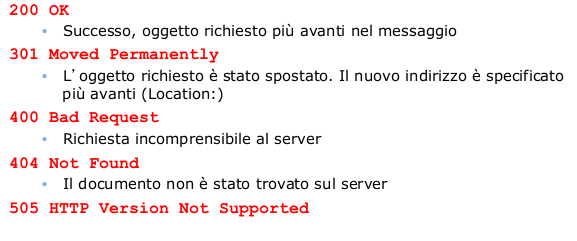
\includegraphics[scale=0.7]{img/http3.png}
\end{figure}
Nonostante il protocollo HTTP è di tipo stateless, per i siti web è comodo poter identificare una persona,
al fine di poter monitorare le abitudini, limitare l'accesso e personalizzare i contenuti, per cui sono 
stati introdotti i \textbf{cookies}, usati di default da tutti i siti.\newline
I cookie prevedono 4 componenti: una header line nel messaggio di risposta HTTP, un header line nel
messaggio di richiesta HTTP, un file di cookie tenuto nel sistema dell'utente e utilizzato dal browser,
infine un database back-end nel sito web.

Per capire come funzionano i cookie guarda la figura \ref{fig:cookie}, in cui si suppone che 
Susan accede al sito di Amazon per la prima volta, utilizzando nel header $Set-cookie: 1678$.\newline
Nonostante i cookie semplificano le procedure di riconoscimento dell'utente, come ad esempio 
si ha la possibilità di usare un applicazione e-mail senza doversi ogni volta registrare, 
ci sono alcuni aspetti negativi riguardo alla privacy, dato che tramite i cookies ed informazioni
ottenute sull'account di un utente, un sito web è in grado di sapere molto sull'utente e può 
vendere a terze parti, cosa che un utente vorrebbe sicuramente evitare.

La web cache, chiamata anche server proxy, è un rete in grado di soddisfare le richieste per conto di un
web server e possiede un suo storage sul disco, per tenere le copie degli oggett richiesti recentemente,
per cui si può configurare, come si nota nella figura \ref{fig:cache}, il browser affinche ogni richiesta 
HTTP venga dirottatta alla web cache, in cui in caso vi sia già una copia dell'oggetto viene subito 
mandata al browser, senza contattare il web server, altrimenti la web cache effettua una HTTP request
al web server e dopo aver ottenuto l'oggetto lo salva internamente e lo manda, tramite una HTTP response,
al browser che lo ha richiesto;come si può notare la web cache agisce sia da client che da server, infatti
quando interagisce con il browser è un server mentre quando comunica con il web server agisce come un client
e solitamente viene acquistata ed installata da un provider ISP.

La cache ha avuto un notevole utilizzo nel campo di internet per due ragione:
\begin{itemize}
    \item può ridurre il tempo di risposta di una richiesta client, in particolare se il collegamento
        tra client e web cache possiede una banda più potente del collegamento tra client e server
        e solitamente ciò avviene, e se si ha un alto tasso di possesso dell'oggetto richiesto da parte
        della cache, al fine di evitare continue richieste al web server.

    \item riduce il traffico sul link di accesso ad internet di una compagnia e/o istituzione, con la
        possibilità di evitare un upgrade della banda, con notevoli risparmi di costi.\newline
        Questa riduzione del traffico fornisce un guadagno anche agli utilizzatori delle applicazioni web
        dato che vi è un miglioramento delle prestazioni.
\end{itemize}
Nonostante la cache riduca il tempo di risposta, introduce il problema sulla integrità della copia
dell'oggetto rispetto a quella nel web server ma per risolvere il protocollo prevede un meccanismo, 
chiamato \textbf{conditional GET}, che permette alla cache di verificare se l'oggetto presente nel
suo storage interno è aggiornato.\newline
Un messaggio HTTP request prevede questo meccanismo in caso il messaggio usa il metodo GET ed 
include l'header \textbf{If-modified-since}, per cui la cache manda l'oggetto richiesto in caso 
in cui l'header if-modified-since coincide con il valore del header last-modified.

Per gestire l'accesso ai documenti sul server, dato che http è stateless, si deve verificare ogni richiesta 
e le informazioni necessarie all'autenticazione si trovano nell'header (\textit{authorization: line}) 
senza le quali il server rifiuta la connessione (\textit{www authenticate:}), come si nota 
nella figura \ref{img:authentication}.
\begin{figure}
    \caption{HTTP authentication}
    \label{img:authentication}
	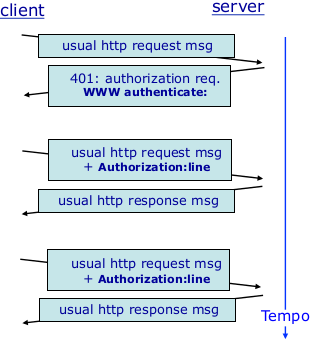
\includegraphics[scale=0.7]{img/http6.png}
\end{figure}

\chapter{HTML + CSS + JS}
Il linguaggio \textbf{HTML} è un linguaggio di markup, per dare struttura ai contenuti web,
utilizzato per annotare un documento in maniera tale che l'annotazione sia sintatticamente
distiguibile dal testo per diverse finalità:
\begin{itemize}
    \item di presentazione, in cui si definisce come visualizzare il testo al quale sono associate.
    \item procedurali, in cui si definiscono istruzioni per programmi che elaborino il testo associato.
    \item descrittive, in cui si etichettano semplicemente parti del testo, 
        al fine di disaccopiare la struttura dalla presentazione del testo spesso.
\end{itemize}
Un esempio di una pagina html si nota nella figura \ref{listato:htmlExample}

\begin{figure}
    \caption{Html example}
    \label{listato:htmlExample}
	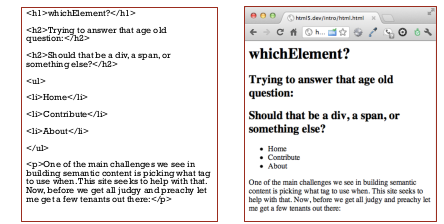
\includegraphics[scale=0.9]{img/html.png}
\end{figure}
Il \textbf{CSS}(Cascading Style Sheets) è un linguaggio per dare uno stile ai contenuti web e la sua specifica
viene definita dal W3C(World Wide Web Consortium), un suo esempio si trova nella figura \ref{css:example}
mentre il DOM(Document Object Model) è un interfaccia neutrale rispetto al linguaggio e alla piattaforma
usata al fine di consentire l'accesso e la modifica dinamica di contenuto, struttura e lo stile di un
documento web, come si nota nella figura \ref{dom:example}.

\begin{figure}
    \caption{Css example}
    \label{css:example}
	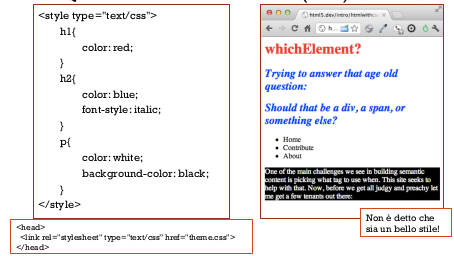
\includegraphics[scale=0.9]{img/css.png}
\end{figure}

\begin{figure}
    \caption{Dom example}
    \label{dom:example}
	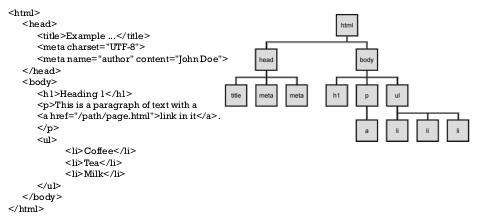
\includegraphics[scale=0.9]{img/dom.png}
\end{figure}
Ogni nodo può essere caratterizzato da attributi per facilitarne l'identificazione, la ricerca, la selezione:
\begin{itemize}
	\item un \textbf{identificatore univoco}, anche se il DOM non garantisce l'unicità
	\item una \textbf{classe} che indica l'appartenenza ad un insieme che ci è utile definire
\end{itemize}
Le \textbf{media query} possono essere viste come particolari selettori capaci di valutare le capacità
del device di accesso alla pagina (schermi, stamparti, text-to-speech), controllando le dimensioni
del device o della finestra, l'orientamento dello schermo e la risoluzione.
Vediamo un esempio:\\
\textit{se la pagina è più larga di 480
	pixel (e si sta visualizzando sullo schermo), applica
	determinati stili agli elementi con id "leftsidebar" (un menu) e "main" (la colonna centrale)}:
\begin{minted}{css}
@media screen and (min-width: 480px){
  #leftsidebar {width: 200px; float: left;}
  #main {margin-left:216px;}
}
\end{minted}
In CSS si ha il termine \textit{cascading} perché esistono potenzialmente diversi stylesheet:
\begin{itemize}
	\item l'autore della pagina in genere ne specifica uno (il modo più comunemente inteso) o più d'uno
	\item il browser ne ha uno, o un vero e proprio CSS o simulato nel loro codice
	\item il lettore, l’utente del browser, ne può definire uno proprio per customizzare la propria esperienza
\end{itemize}
Dei conflitti sono quindi inevitabili per cui è necessario definire un algoritmo per decidere quale
stile vada applicato a un elemento.\newline
Si ha il seguente ordine di importanza dei seguenti fattori associati alle regole:
\begin{enumerate}
	\item \textbf{importanza} (flag specifico \textit{!important} per un attributo)
	\item \textbf{specificità} (per esempio, \textit{id > class > tag})
	\item \textbf{ordine nel sorgente }(il più “recente” vince)
\end{enumerate}
Il browser non è solamente un banale visualizzatore di pagine scritte in HTML, è un vero e proprio 
ambiente di sviluppo (in particolare contiene un interprete Javascript e vari strumenti di debug,
ma ne parleremo più avanti) che fornisce numerose funzionalità abilitanti inoltre l'impostazione di
HTML e CSS separa nettamente il contenuto dalla modalità di visualizzazione.\newline
Esistono numerosi "front-end framework", dai più sofisticati ai più semplici, naturalmente open source, ad esempio:
\begin{itemize}
	\item \textbf{bootstrap}
	\item \textbf{foundation}
	\item \textbf{skeleton}
\end{itemize}

\subsection{HTML5}
HTML5 ha introdotto nuovi \textbf{elementi semantici} per la strutturazione delle pagine, per esempio:
\begin{itemize}
	\item article
	\item section
	\item aside
	\item header
	\item footer
\end{itemize}
Introduce inoltre nuovi \textbf{elementi di input e multimediali}, widget per input search, email,
url, number, tel, ma anche range, date \dots,  anche se il supporto a tutto ciò da parte dei browser non è uniforme.

L’HTML dovrebbe non contenere informazione di presentazione, riservata ai CSS, 
quindi senza stili definiti "in linea" e senza l'uso di tag come <font>, <b>, <i> ma dovrebbe solo 
occuparsi delle informazioni da volere rappresentare nel file web.

HTML5 sia più leggibile. In generale, a parte essere una notazione più concisa e che richiede
meno definizioni di classi, le gerarchie di contenuti più leggibili e analizzabili 
in fase di progettazione, manutenzione e debug.

Per avere informazioni riguardo alla sintassi html e css si consiglia di guardare i tutorial presenti 
in internet su W3CSchool.

\end{document}
